\documentclass[twoside]{article}
\input{ISC18-english.sty}
%%%%%%%%%%%%%%%%%%%%%%%%%%%%  Make sure to compile twice for proper cross-references. %%%%%%%%%%%%%%%%%%%%%%%
%%%%%%% For proper display of references, compile the document twice. %%%%%%%%%%%%%%%%%%%%% 
%%%%%%%%%%%%%%% If using TeX Live, compile using pdflatex command %%%%%%%%%%%%%%%%%%%%%%%
\begin{document}
\thispagestyle{empty}
%%%%%%%%%%%%%%%%% Article title header  %%%%%%%%%%%%%%%%%%%%
\fancyhead[LE]{Evidential sets for the circular normal distribution}
%%%%%%%%%%%%%%%%% Article authors header   %%%%%%%%%%%%%%%%%%%%
\fancyhead[RO]{Sarvari, Doostparast and Emadi}
\begin{center}
{
\includegraphics [height=25mm, width=150.3mm] {Images/isc18E}} \\
\vspace*{-1.8cm}
%\begin{center}
%\color{blue} 
%{\hspace{0.1cm}\rule{\textwidth}{1mm}}\\
%\end{center}
\vspace*{4cm}
%%%%%%%%%%%%%%%%% Article title  %%%%%%%%%%%%%%%%%%%%
{\Large \bf Evidential sets for the circular normal distribution}\\
%%%%%%%%%%%%%%%%% Article authors and affiliations %%%%%%%%%%%%%%%%%%%%
{\bf MohammadReza Sarvari\footnote[1]{{\bf Corresponding Author:} {\tt sarvari.mohammadreza@mail.um.ac.ir}}, Mahdi Doostparast$^2$,  Mahdi Emadi$^3$ \\
$^1$$^2$$^3$Department of Statistics, Ferdowsi University , Mashhad , Iran. }
%$^2$Department of Statistics, Ferdowsi University , Mashhad , Iran.\\
%$^3$Department of Statistics, Ferdowsi University , Mashhad , Iran.}
\end{center}
\rule{\textwidth}{0.2mm}\\
%%%%%%%%%%%%%%%%% Article abstract  %%%%%%%%%%%%%%%%%%%%
\noindent{\bf Abstract:}\\
Directional data arise in various applied fields, such as wind directions, daily event times, and bird flight directions. This paper addresses evidential intervals for directional data within the evidential inference framework. To this do, a sample coming from the circular normal distribution is assumed. Intervals for the population parameters are considered when the concentration parameter is either known or unknown. For large sample sizes, some approximations are also provided to enable fast computations with massive datasets. The performance of the proposed results is illustrated by analyzing a real dataset on the times of urban injury accidents.
 
\noindent{\bf Keywords:} 
 Likelihood Ratio, Circular and Directional Data, Evidential interval, Evidential sets.\\
\noindent{\bf Mathematics Subject Classification (2020):} $\rm 62F25$, $\rm 62H11$, $\rm 62F15$. \\
\hspace{1cm}\rule{\textwidth}{0.2mm}\\
%%%%%%%%%%%%%%
\section{Introduction}
In various scientific fields, measurements often take the form of directions. For example, a biologist might study the flight direction of birds or the orientation of an animal, while a geologist may be interested in the direction of Earth's magnetic pole. Some of these measurements are two-dimensional, like the first two examples, while others, like the last, are three-dimensional.

A collection of such observations is known as directional data (\cite{JS2001}). Two-dimensional directions are represented as angles measured from a chosen "zero direction" and a specified sense of rotation (clockwise or counterclockwise). Since directions lack magnitude, they can be conveniently represented as points on the circumference of a unit circle centered at the origin, or as unit vectors from the origin to those points. Due to this circular representation, two-dimensional directional data are also called circular data.

Directional data present unique modeling and statistical challenges. For instance, the numerical representation of a direction as an angle is not unique because it depends on the choice of zero direction and the sense of rotation. Moreover, an angle of 60° according to a mathematician (using East as zero and counterclockwise as positive) corresponds to 30° for a geologist using North as zero and clockwise as positive—the latter is called the "azimuth." Just as the normal distribution is fundamental for linear data, the circular normal (CN) distribution is essential for analyzing directional data. 

\begin{dfn}\label{df1}
A random variable $Z$ is said to have the CN distribution, denoted by $Z \thicksim CN(\mu, \nu)$,  if it has the density function
\begin{equation} \label{pdf:CN}
 f(z;\mu, \nu)=\frac{1}{2\pi I_{0}(\nu)} \exp{\lbrace \nu \cos(z -\mu)\rbrace},\ 0 \leq z \leq 2\pi,\ \ 0\leq  \mu \leq 2\pi,\ \ \nu > 0,
\end{equation}
\end{dfn}

where $I_{0}(\nu)$ is the modified Bessel function of the first kind and order zero; that is,
\begin{equation}\label{eq1}
I_{0}(\nu)=\frac{1}{2\pi}\int_{0}^{2\pi}\exp(\nu \cos(z))dz.
\end{equation}

It is easy to verify that the CN distribution is symmetric and has a mode at the mean $\mu$. The larger the value of $\nu$, the larger will be the ratio of $f(\mu)$ to $f(\mu \pm \pi)$, indicating higher concentration towards the population mean direction $\mu$; see Figure \ref{twocric}.

\begin{figure}[ht]
\begin{center}
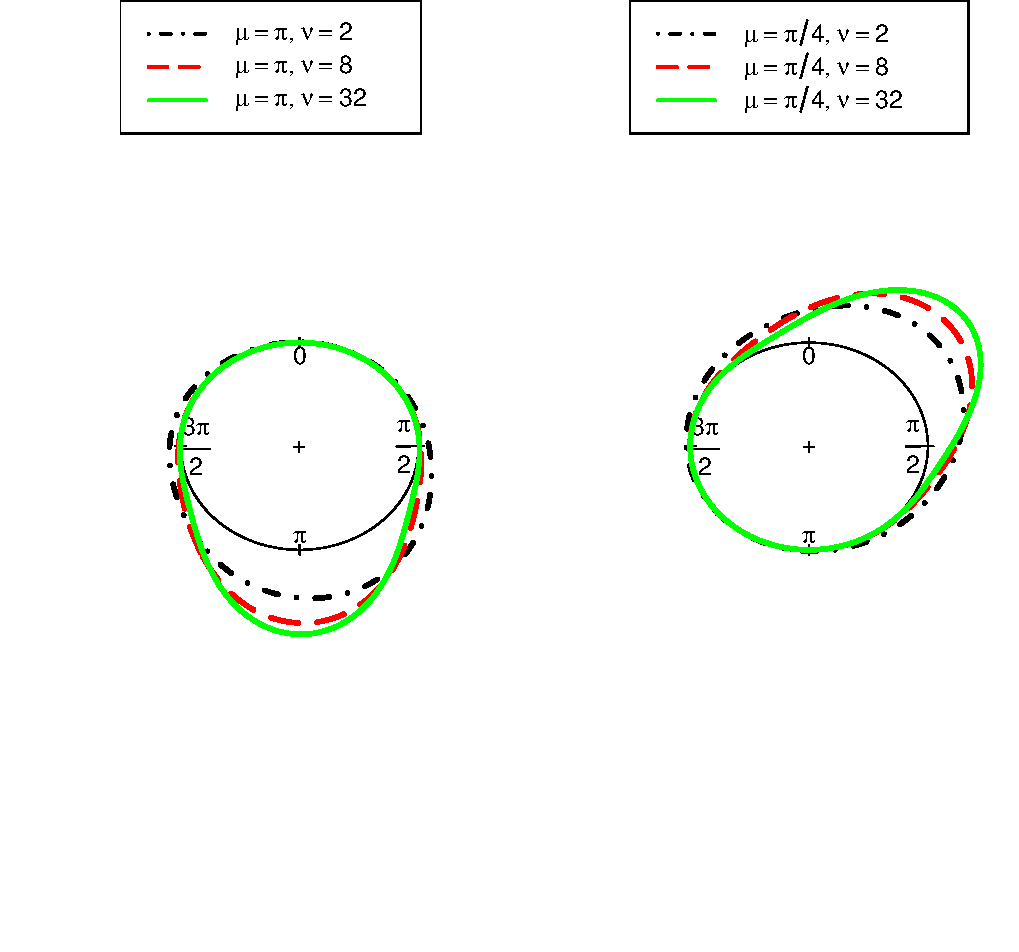
\includegraphics[width=7cm,height=7cm]{Images/twocircle-eps-converted-to.pdf}
\vspace{-3cm}
\caption{\footnotesize{The CN distribution for some selected values of $\mu$ and $\nu$.}}\label{twocric}
\end{center}
\end{figure}
\cite{G1953} called it the "circular normal distribution" due to its similarities to the normal distribution. Since \cite{vM1918} introduced it, it is also known as the von Mises distribution; the two terms are used interchangeably. Statistical inference for this distribution has been extensively developed (e.g., \cite{JS2001}; \cite{M1972}; \cite{SD2026a}).
Testing hypotheses about a population based on data is a fundamental problem. Two common approaches are the Neyman–Pearson decision-theoretic and Bayesian approaches (\cite{LR2005}). The former assumes an action (accepting a hypothesis) incurs a loss if incorrect. The Bayesian approach uses prior probabilities about the hypotheses, updated with data to obtain posterior probabilities. However, both approaches require specifying either loss functions or prior probabilities, which are often unknown. In recent decades, an evidential inference approach has emerged. It relies solely on the likelihood ratio (LR), which quantifies the relative evidence in the data for one hypothesis against another, expressed as odds. This approach avoids the need for loss functions or prior probabilities, complementing classical and Bayesian methods (\cite{R1997}; \cite{EA2003}).


\section{Evidential Inference}
As noted in Section 1, a new approach known as evidential inference has emerged in the literature over recent decades. This approach requires neither a loss function nor a prior probability. Instead, it addresses the extent to which the observed data support competing hypotheses (see, e.g., \cite{R1997}; \cite{EA2003}).
In essence, evidential inference relies solely on the objective component of Bayes' theorem—namely, the likelihood ratio (LR). The LR quantifies the relative evidence in the data for one hypothesis against another and is easily interpreted in terms of odds. For example, based on the evidence, one can readily state that one outcome is ten times more likely than another.
Although the LR is straightforward to understand, we also use its natural logarithm, called the support and denoted by  $S$, because it represents the weight of evidence on a linear scale from $-\infty$ to $+\infty$.


\section{Evidential sets: A general framework}
The likelihood principle is that all the evidence obtained in a study about a measure of interest is contained in the likelihood function (LF) for the data. 
\begin{dfn} 
Let $\mathbf{X}$ follow the probability density function $f_\mathbf{X}(x; \mathbf{\theta})$ for $\mathbf{x}\in S_\mathbf{X}$ and $\mathbf{\theta}\in\mathbf{\Theta}$, where $S_\mathbf{X}$ and $\mathbf{\Theta}$ are the support of $\mathbf{X}$ and the parameter space, respectively. The likelihood function (LF) is defined by
\begin{equation} \label{Likely}
L(\mathbf{\theta}; \mathbf{x})=f_\mathbf{X}(\mathbf{x};\mathbf{\theta}), \ \ \ \forall\mathbf{\theta}\in\mathbf{\Theta},\mathbf{x}\in S_\mathbf{X}.
\end{equation}
\end{dfn}

\begin{dfn} Let $\theta_1$ and $\theta_2$ be two distinct values in $\mathbf{\Theta}$. The likelihood ratio (LR) of $\theta_1$ against $\theta_2$ is defined by
\begin{equation} \label{LR12}
LR_{1|2}=\frac{L(\theta_1; \mathbf{x})}{L(\theta_2; \mathbf{x})}.
\end{equation}
\end{dfn}
The LR in Equation \eqref{LR12} gives us the relative evidence from the collected data for the simple hypothesis $H_1:\mathbf{\theta}=\theta_1$ against the alternative simple hypothesis $H_2:\mathbf{\theta}=\theta_2$ and is easily understood in terms of odds. 
For example, for $LR_{1|2}=2$, we would say that the evidence for $\theta_{1}$ is twice that for $\theta_{2}$. If their likelihoods are the same that would give us an LR of 1, then the evidence did not favour either of $\theta_1$ and $\theta_2$. Finally, if $LR_{1|2}$ is 0.5, then we say that the evidence for $\theta_{1}$ is half of that for $\theta_{2}$, or alternatively, that there is twice as much evidence favouring $\theta_{2}$ over $\theta_{1}$.

Evidence is represented by the LR at least some threshold value $k$. The observations are strong evidence in favour of $H_1$ if $LR_{1|2}\geq k$, strong evidence in favour of $H_2$ if $LR_{1|2}\leq 1/k$, and weak evidence if $1/k < LR_{1|2} < k$. With this in mind, the evidential set at level $k$ is defined.
\begin{dfn}\label{def:evidential:set:general}
The evidential set at level $k$ for $\mathbf{\theta}$, denoted by $EI_k(\mathbf{\theta})$, based on the observed data $\mathbf{x}$ is defined by
\begin{equation}\label{EIk:general}
EI_k(\mathbf{\theta})=\left\{\mathbf{\theta}:\frac{L(\mathbf{\theta};\mathbf{x})}{L(\hat{\mathbf{\theta}};\mathbf{x})}\geq \frac{1}{k}\right\},
\end{equation}
where $\hat{\mathbf{\theta}}$ is the maximum likelihood estimation (MLE) of the parameter $\mathbf{\theta}$, i.e.
\[\hat{\mathbf{\theta}}=\arg\max_{\mathbf{\theta}\in\mathbf{\Theta}} L(\mathbf{\theta};\mathbf{x}). \]
\end{dfn}
%Notice that the evidential sets in Equation \eqref{EIk:general} are not confidence sets, in general. Rather, they truly represent what confidence sets are often mistaken to represent: namely, parameter values that the sample does not provide evidence against. In other words, these are values that are ``consistent with the observations." One can say in this way that there is not strong evidence against a point inside the evidential set, without reference to an alternative value. This claim holds because it is true for all alternative values simultaneously. For more details, see \cite{R1997}.
%For example, every point inside the evidential set at level $k=8$ is consistent with the observations in the strong sense that there is no other possible value of the parameter that is better supported by a factor as large as 8.
%For points outside the evidential sets, the interpretation must be more careful. There is fairly strong evidence against a point just outside the 1/8 likelihood interval in the specific sense that there is some alternative value, namely the MLE that is better supported by a factor at least 8. For more details, see \cite{R1997}.

%\begin{remark}
%What value of $k$ is appropriate? The question is analogous to the one that is asked in problems of hypothesis testing: ``what significance level is appropriate?'' Although no one choice will work for all problems, \cite{R1997} established useful guidelines and conventions. Indeed, the $5\%$ significance level has been widely accepted as identifying evidence of sufficient strength to be of general scientific interest. In the same way, a LR of 8 is suggested. When ``quite strong" evidence is sought, conventionally expressed  by the choice of the $1\%$ significance level, one might choose a threshold $k=32$. 
%\end{remark}
%
%\begin{remark}
%Based on the evidence, it is easy to consider one outcome being ten times more likely than another. Although the LR is easily grasped, one can also use the natural log of the LR, called the support. It represents the weight of evidence on a linear scale from $-\infty$ to $+\infty$. The support function has distinct advantages over the LR function; see, for example,\cite{R1997}, and Cahusac (2021). 
%\end{remark}

\subsection{Parameter estimates for the CN distribution}
In the following, the CN distribution is explained, followed by some findings from that distribution.. Let $\mathbf{Z}=(Z_1, \ldots, Z_n)$ be a random sample coming from the $CN(\mu,\nu)$ distribution and  let $\mathbf{z}=(z_1,\ldots, z_n)$ be the observed value of $\mathbf{Z}$. 
The likelihood function (LF) is obtained from Equation \eqref{pdf:CN} as
\begin{equation}\label{LF:CN}
L(\mu, \nu ; \mathbf{z})= \frac{1}{(2\pi I_{0}(\nu))^n} \exp{\left(\sum_{i=1}^{n}\nu \cos(z_{i}-\mu)\right)},  ~~~~~ 0\leq \mu < 2\pi, \nu > 0,
\end{equation} 

and thus the logarithm of LF (LLF) is
\begin{eqnarray}\label{LLF:CN}
\ell(\mu, \nu ;\mathbf{z}) &=&\log L(\mu, \nu ;\mathbf{z}) \nonumber \\
&=& -n\ln(2\pi I_{0}(\nu)) +\nu \sum_{i=1}^{n}\cos(z_{i}-\mu).  
\end{eqnarray}
\cite{JS2001} obtained that the maximum likelihood estimate (MLE) of $\mu$ is $\widehat{\mu}=\bar{z}$, where
\begin{eqnarray} \label{mle-mu}
\bar{z}=\arctan^*\left(\frac{S({\mathbf{z}})}{C({\mathbf{z}})}\right)=
\begin{cases}
\arctan \left(\frac{S({\mathbf{z}})}{C({\mathbf{z}})}\right), & \hspace{0.5cm} C({\mathbf{z}})>0, S({\mathbf{z}}) \geq 0, \\
\frac{\pi}{2}, & \hspace{0.5cm} C({\mathbf{z}})=0, S({\mathbf{z}})>0, \\ 
\arctan\left(\frac{S({\mathbf{z}})}{C({\mathbf{z}})}\right)+\pi, &\hspace{0.5cm} C({\mathbf{z}})<0, \\
\arctan\left(\frac{S({\mathbf{z}})}{C({\mathbf{z}})}\right)+2\pi, &\hspace{0.5cm} C({\mathbf{z}})\geq 0, S({\mathbf{z}})<0, \\
$undefined$, &\hspace{0.5cm} C({\mathbf{z}})=0, S({\textbf{z}})=0,\label{hat{mu}}
\end{cases}
\end{eqnarray}
\begin{equation*}
C({\textbf{z}})=\frac{1}{n}\sum_{i=1}^{n}\cos (z_{i}), \;\;\;\;\;\;\;\;\;\;\  S({\textbf{z}})=\frac{1}{n}\sum_{i=1}^{n}\sin (z_{i}).
\end{equation*}
and

The MLE of $\nu$ is $\widehat{\nu}=A^{-1}(\bar{R})$
%\begin{equation}\label{hat{nu}}
%\widehat{\nu}=A^{-1}(\bar{R}),
%\end{equation}
where
$\bar{R}=n^{-1}\sum_{i=1}^n \cos(z_{i} -\bar{z})$,  $A(\nu)={I_{1}(\nu)}/{I_{0}(\nu)}$, $I_0(\nu)$ is given by Equation  \eqref{eq1} and 

\[I_{1}(\nu)=\frac{\partial I_{0}(\nu)}{\partial \nu}= \frac{1}{2\pi} \int_{0}^{2\pi} \cos(z)\exp\left(\nu \cos(z)\right)dz.\] 
%%%%%%%%%%%%%%%%%%%%%%%%%%%%%%%%%%%%%%%%%%%%%%%%%
\section{Evidential interval for direction mean ($\mu$) in CN distribution}
In this section, the evidential intervals are derived on the basis of a random sample coming from CN distribution.
\begin{lem}
The MLE $\hat{\mu}=\bar{z}$ in Equation \eqref{mle-mu} is rotationally equivariant, i.e., if the data is rotated by a certain amount, the value of $\bar{z}$ also changes by the same amount.
\begin{eqnarray}
\sum_{i=1}^{n} \cos(z_i + constant)=R \cos(\bar{z}+constant).
\end{eqnarray}
that $ R=\sqrt{C^2+S^2}$.
\end{lem}
\begin{proof}
 For more details, see \cite{JS2001}.
\end{proof}
\begin{pro}
If $\nu$ is known, the evidential interval for $\mu_0$ at level $k$ is
\begin{eqnarray} \label{SIE}
\bar{z}-  \left| \arccos(\frac{\sum_{i=1}^{n} \nu_0 \cos(z_i + \bar{z})-\ln(k)}{R \nu_0 })\right| < \mu_0  < \bar{z} +\left| \arccos(\frac{\sum_{i=1}^{n} \nu_0 \cos(z_i + \bar{z})-\ln(k)}{R \nu_0 })\right| .
\end{eqnarray}
\end{pro}
The proof the above propostion is given by \cite{SDM2026b} in details.

For the unknown $\nu$, one can easily plug-in the estimates of the parameters into Equation (3.2). Meanwhile, an alternative approach is provided by \cite{SDM2026b}.
\section{Illustrative examples} 
Traffic accidents and urban road incidents resulting in injuries or fatalities are among the serious challenges facing modern societies. These events are typically caused by various factors, including speeding, failure to obey traffic laws, vehicle malfunctions, driver distractions (such as mobile phone use), and inadequate road infrastructure. In cities, the high density of vehicles and the complex interactions between cars, motorcycles, bicycles, and pedestrians increase the likelihood of accidents. The consequences of such accidents include loss of life, physical and psychological injuries, as well as significant ec2onomic and social costs to the community. Preventing these incidents requires a comprehensive approach that encompasses public education, infrastructure improvements, enforcement of regulations, and the promotion of a safe driving culture.
%Traffic and urban road accidents leading to injuries or fatalities are among the serious challenges in modern societies. These incidents are typically caused by various factors, such as speeding, failure to adhere to traffic laws, vehicle malfunctions, driver distractions (such as mobile phone use), and inadequate road infrastructure. In cities, the high density of vehicles and the complex interactions between cars, motorcycles, bicycles, and pedestrians increase the likelihood of accidents. The consequences of these accidents include loss of life, physical and psychological injuries, and significant economic and social costs to the community. Preventing such incidents requires a comprehensive approach, including public education, infrastructure improvements, enforcement of regulations, and the promotion of a culture of safe driving.

In this section, a data set about the  time of $n=42$ injury accidents on an urban road in Iran from 2012 to 2016 is analyzed using the results obtained  in the preceding sections. The variable of interest here is the time of occurrence of the accident during 24 hours of a day,  {with the period of $\displaystyle \frac{\pi}{12}T$ where $T=\lbrace 1,2,\ldots, 24\rbrace$}. Table \ref{tab:data} presents the data set.

\begin{table}[!htp] 
\centering
\caption{Times of injury accidents in an urban road in Iran from 2012 to 2016.} \label{tab:data}
\begin{tiny}
\begin{tabular}{cccccc} 
\hline \hline
20:44:04 &   21:44:28 &  07:49:11 &   09:17:15  &   16:41:13 &    20:35:03 \\
   03:23:58 &   17:39:01 &   17:58:09 &   19:00:31 &   23:18:32 &   01:08:29   \\
   18:06:54   &  00:00:00 &   00:00:00 &   16:50:00 &   18:30:00 &   08:45:00 \\
    00:00:00 &   07:36:05 &   00:24:42 &   22:37:36 &   09:35:29 &   22:22:12 \\
    16:12:01 &    09:37:10 &     10:11:43  &    23:33:13 &   14:29:21  & 22:29:14 \\
   17:00:22 &    16:26:00 &   02:26:59 &    07:36:05 &    00:24:42 & 22:37:36 \\
19:37:07 & 12:46:43 &  22:49:21 & 00:00:00 &  18:00:00  & 01:26:00  \\
\hline \hline
\end{tabular}
\end{tiny}
\end{table} 

To visualize the circular data set in Table \ref{tab:data}, the mathematical software $\mathsf{MAPLE}$ 2023 version was used.
\begin{figure}[ht]
\begin{center}
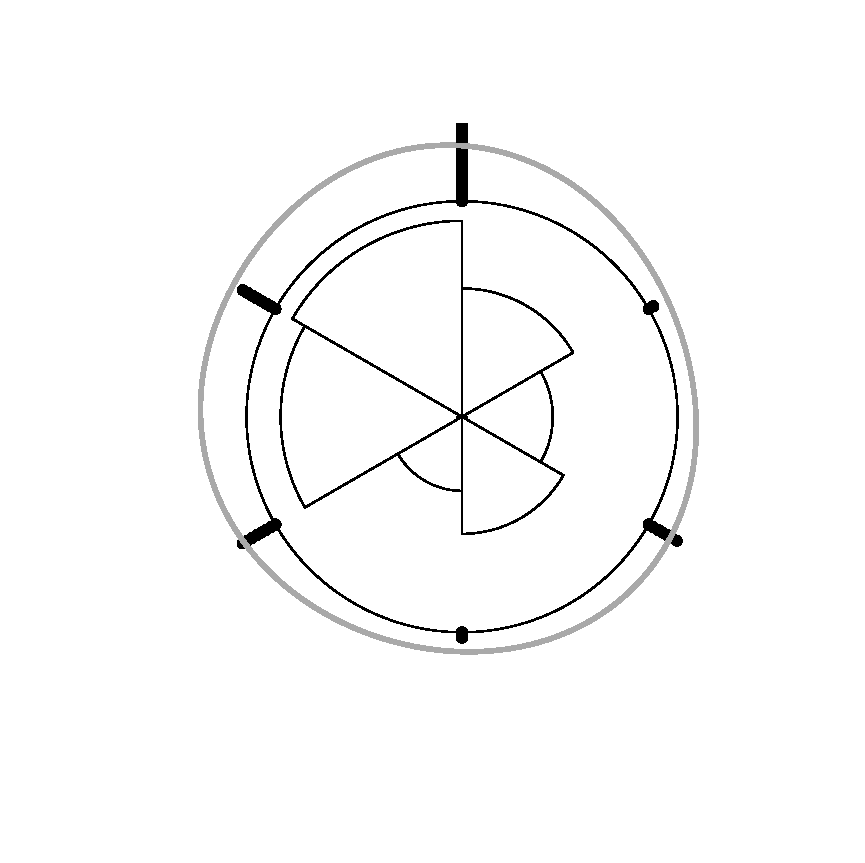
\includegraphics[width=5cm,height=5cm]{Images/figcircle-eps-converted-to.pdf}
\vspace{-2cm}
\caption{\footnotesize{The raw circular plot, the rose diagram, and the kernel density estimation for the data set in Table \ref{tab:data}.}}\label{fig1}
\end{center}
\end{figure}
Figure \ref{fig1} displays the raw circular plot and the respective rose diagram. Rose diagrams are more informative than circular plots. The areas of the sectors in the given rose diagram in Figure \ref{fig1} represent the relative frequencies in the  24 class intervals. As one can see,   most accidents occur during   evening and midnight. Also, the kernel density estimation for times of injury accidents on the basis of the data set in Table \ref{tab:data} is provided in Figure \ref{fig1}. In fact,  the most suitable visualization tool for displaying circular data is the kernel density chart; see, for example, \cite{P2013} and references therein. Note that the circular mean of the accident times in Table \ref{tab:data} is $C({\textbf{z}})=\frac{1}{n}\sum_{i=1}^{n}\cos (z_{i})$ , $S({\textbf{z}})=\frac{1}{n}\sum_{i=1}^{n}\sin (z_{i})$, since $S<0$, the Equation $\eqref{mle-mu}$ implies that the mean is  arctan$(\frac{S({\textbf{z}})}{C({\textbf{z}})})+2pi$, which is equivalent to 9:18:52 PM, while the arithmetic mean is 3.37778, which is equivalent to 12:54:07 PM. This states that considering linear methods for analysing this circular data set may concludes bias results and be misleading. For more details, see \cite{M1972} \cite{MJ2001}, \cite{P2013}, \cite{SD2026a}, and the references therein.

Traffic experts believe that accidents occur commonly at night. In what follows, we are interested to obtain an interval for the direction mean parameter $\mu$ by assuming the $CN(\mu, \nu)$ distribution for the population if the accident times. 
%First, to assess the adequacy of the CN distribution for the accident times in Table \ref{tab:data}, the goodness-of-fit test was performed by the $\mathsf{watson.test}$ procedure in the $\mathsf{circular}$ package of the $\mathsf{R}$ software version 4.3.3. {For more details, see Pewsey et al. (2013)}. It was confirmed that the data follows the CN distribution. So, the problem of interest can be phrased as a hypothesis problem based on the parameters of the CN distribution.
%\section{Real eample for support interval}
Evidential interval for sample sizes with $n = 42$ injury accidents on an urban road in Iran from 2012 to 2016 is analyzed using the results obtained in the preceding sections.
The left figure \ref{LRTkpi2} displays an evidential interval from $-\pi$ to $\pi$. 

Or the same the right figure \ref{LRTkpi2} displays an evidential interval from $0$ to $2\pi$, because the circular data are on circular axis. 
\begin{figure}[ht]
\begin{center}
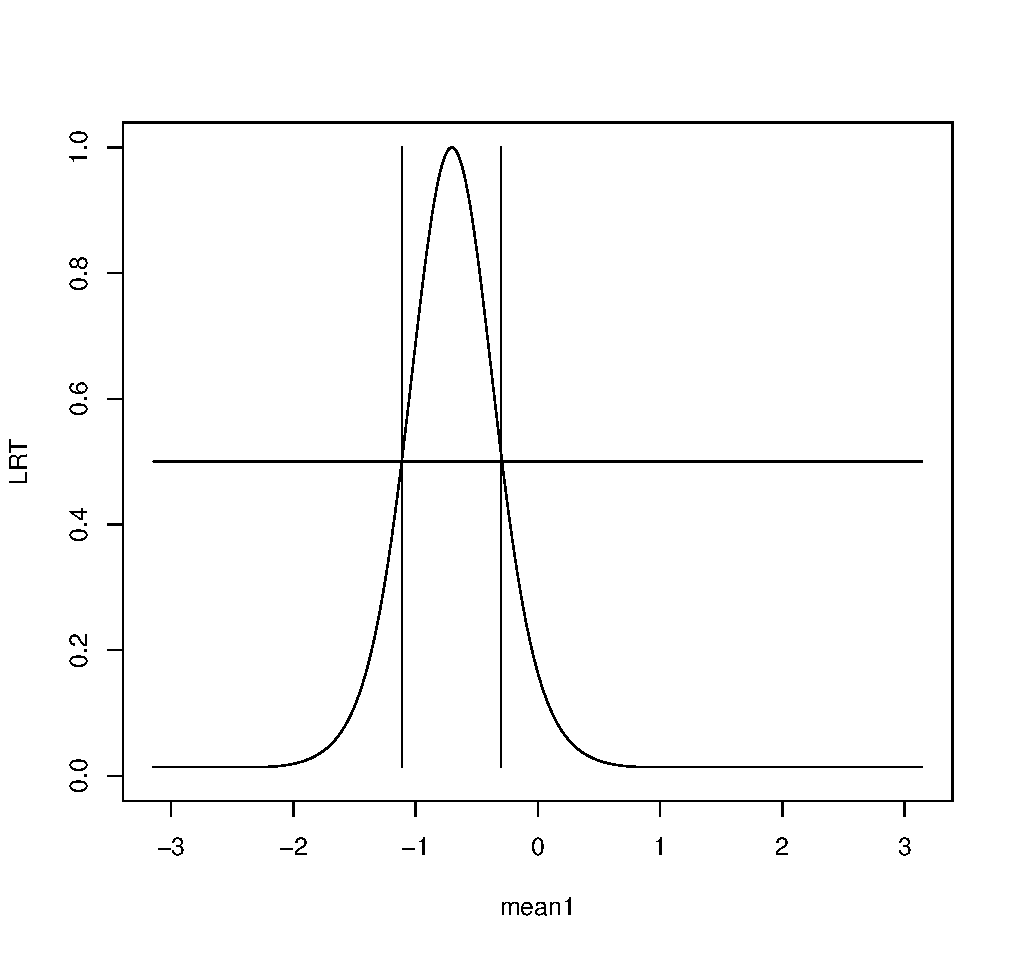
\includegraphics[width=5cm,height=4cm]{Images/LRT,k=0.5-eps-converted-to.pdf}
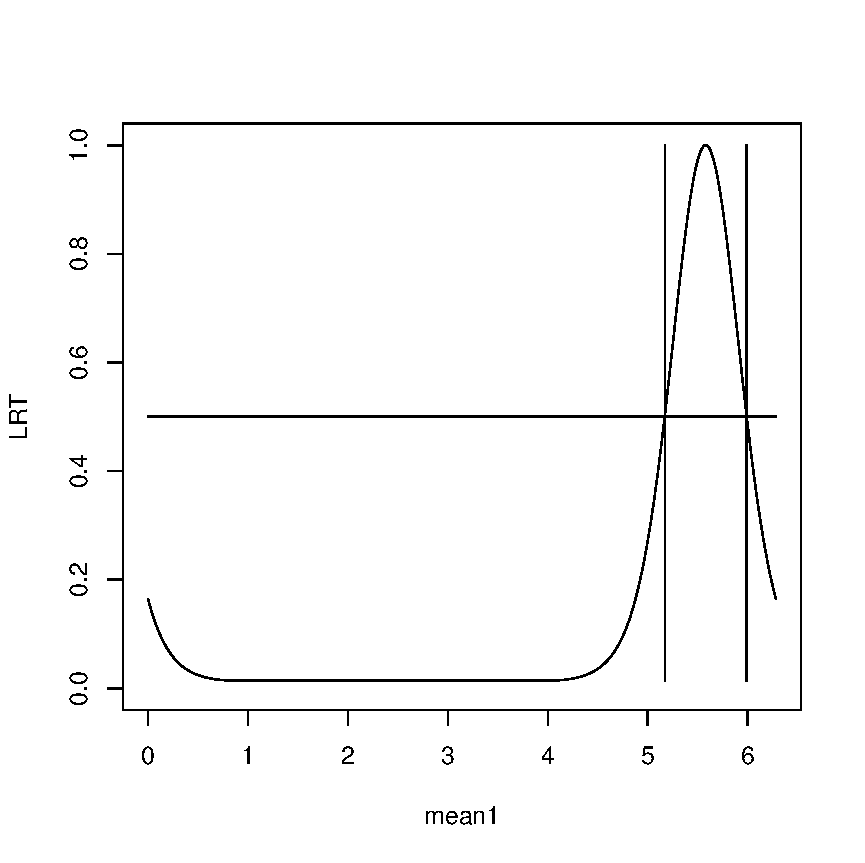
\includegraphics[width=5cm,height=4cm]{Images/LRT1,k=0.5-eps-converted-to.pdf}\\
\vspace{-0.5cm}
\caption{\footnotesize{For the data set in Table \ref{tab:data}, an evidential interval (with $k>1/2$) is displayed. This interval ranges from $-\pi$ to $\pi$ with a lower bound of $-1.112647$ and a upper bound of $-0.3010693$. Alternatively, when mapped to the interval from $0$ to $2\pi$, the same evidential interval is expressed with a lower bound of $-1.112647+2\pi=5.170538$ and a upper bound of $-0.3010693+2\pi=5.982116$.
}}\label{LRTkpi2}
\end{center}
\end{figure}

\section*{Discussion and Conclusion}   
The evidential approach was used for interval estimation of the mean direction parameter, with approximations based on the law of large numbers and the CLT for fast computation on massive datasets. Unlike classical and Bayesian methods, this approach requires neither a loss function nor a prior, thus avoiding personal opinions of researchers. Possible extensions include wrapped normal, circular uniform, wrapped Cauchy, and multivariate spherical distributions.
\section*{Acknowledgments}   
The author would like to express sincere gratitude to his supervisor and advisor for their invaluable guidance and support in the preparation of this conference paper. He also thanks the Eighteenth Iranian Statistical Conference hosted by Khajeh Nasir Toosi University of Technology.
\begin{thebibliography}{9}
\bibitem[Emadi and Arghami (2003)]{EA2003}
Emadi M. and Arghami N. R. (2003), Some Measure of Support for Statistical Hypotheses, {\it Journal of Statistical Theory and Applications}, 2(2), 165--176.
\bibitem[Gumble et al. (1953)]{G1953}
Gumble E. J., Greenwood J. A. and Durand D. (1953), The circular normal distribution: Theory and tables, {\it Journal of the American Statistical Association},48(261), 131--152.
\bibitem[Jammalamadaka and Sengupta (2001)]{JS2001}
Jammalamadaka S. R. and Sengupta A. (2001), {\it Topics in circular statistics,} World Scientific, \textbf{5}. London.
\bibitem[Lehmann and Romano (2005)]{LR2005}
Lehmann E. L. and Romano J. P. (2005), {\it Testing Statistical Hypotheses,} Second edition, Springer, New York.
\bibitem[Mardia (1972)]{M1972}
Mardia K.V. (1972),{\it Statistics of Directional Data,} Academic Press, New York.
\bibitem[Mardia and Jupp (2001)]{MJ2001}
Mardia K. V. and Jupp P. E. (2001), {\it Directional statistics,} 2nd Edition, John Wiley \& Sons, New York.
\bibitem[Pewsey et al. (2013)]{P2013}
Pewsey A., Neuhäuser M. and Ruxton G. D. (2013), {\it Circular statistics in R,} OUP Oxford, United Kingdom.
\bibitem[Royall (1997)]{R1997}
Royall R. M. (1997), {\it Statistical Evidence: A Likelihood Paradigm,} Chapman $\&$ Hall, London.
\bibitem[Sarvari and Doostparast (2026a)]{SD2026a}
Sarvari M. R. and Doostparast M. (2026a), Evidence in directional data coming from circular normal distribution, {\it Journal of Applied Statistics}, 53(9), 1733--1759.
\bibitem[Sarvari et al. (2026b)]{SDM2026b}
Sarvari M. R., Doostparast M. and Emadi M. (2026b), Evidential sets based on directional observations from circular normal
distributions, working.
\bibitem[von Mises (1918)]{vM1918}
von Mises, R. (1918), Über die “Ganzzahligkeit" der atomgewichte und verwandete fragen, {\it Physikalische Zeitschrift} 19, 490-500.
\end{thebibliography}
 \end{document}

